%!TEX encoding = UTF-8 Unicode

% this figure should come before the proposed approach section.
% It might happen automatically if we shorten the introduction.
% Otherwise move back in the files.
%\newcommand{\myWidth}{0.22}
\newcommand{\myWidth}{0.16}
\begin{figure*}
  \centering
  \subfloat[][Grasp: the human moves the hand towards an object vertically, then grasps and lifts it.]{
    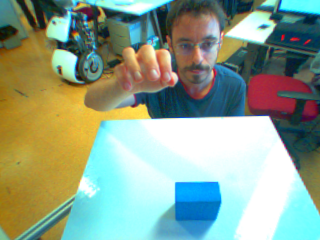
\includegraphics[width=\myWidth\linewidth]{grasp-00000169}
    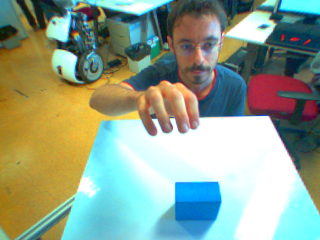
\includegraphics[width=\myWidth\linewidth]{grasp-00000170}
    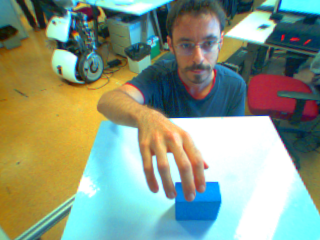
\includegraphics[width=\myWidth\linewidth]{grasp-00000171}
    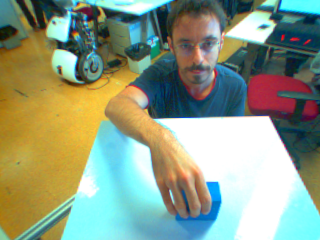
\includegraphics[width=\myWidth\linewidth]{grasp-00000173}
    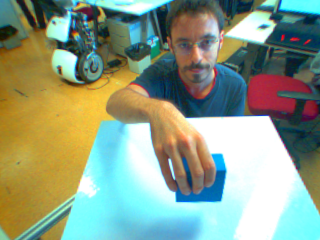
\includegraphics[width=\myWidth\linewidth]{grasp-00000177}
    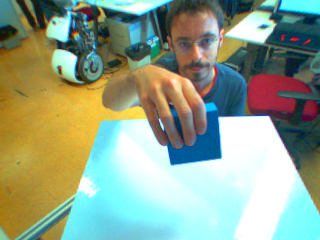
\includegraphics[width=\myWidth\linewidth]{grasp-00000180}
    \label{fig:action_examples:grasp}
  } % end subfloat

  \subfloat[][Tap: the human moves the hand towards an object laterally and touches it, causing a motion effect.]{
    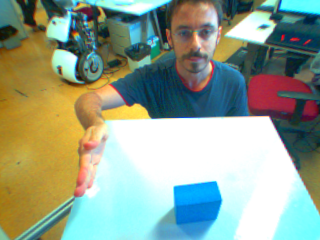
\includegraphics[width=\myWidth\linewidth]{tap-00000109}
    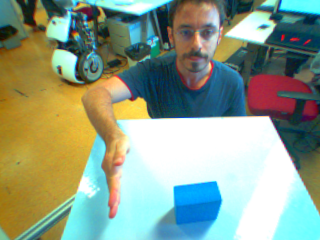
\includegraphics[width=\myWidth\linewidth]{tap-00000110}
    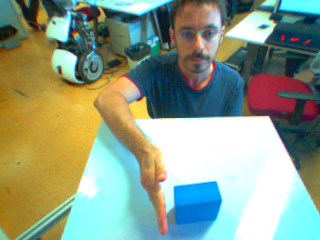
\includegraphics[width=\myWidth\linewidth]{tap-00000112}
    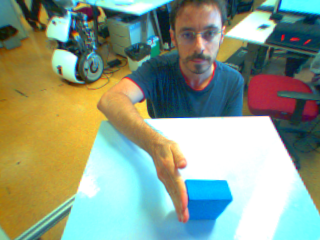
\includegraphics[width=\myWidth\linewidth]{tap-00000114}
    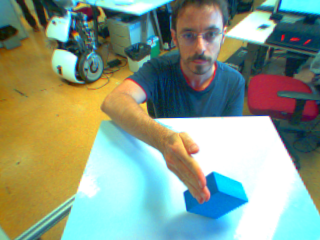
\includegraphics[width=\myWidth\linewidth]{tap-00000116}
    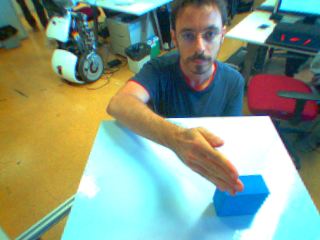
\includegraphics[width=\myWidth\linewidth]{tap-00000117}
    \label{fig:action_examples:tap}
  } % end subfloat

  \subfloat[][Touch: the human moves the hand towards an object vertically, then touches it~(without grasping), then retracts the hand.]{
    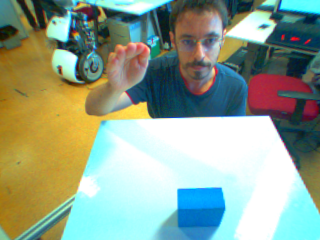
\includegraphics[width=\myWidth\linewidth]{touch-00000196}
    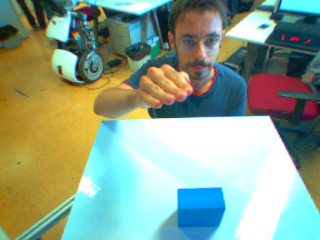
\includegraphics[width=\myWidth\linewidth]{touch-00000197}
    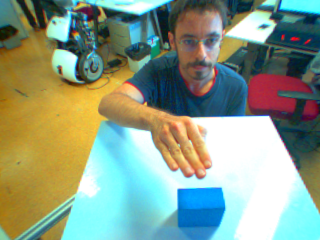
\includegraphics[width=\myWidth\linewidth]{touch-00000198}
    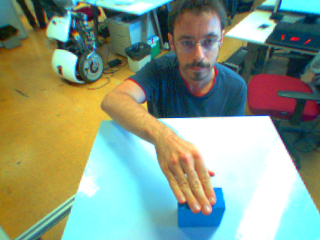
\includegraphics[width=\myWidth\linewidth]{touch-00000200}
    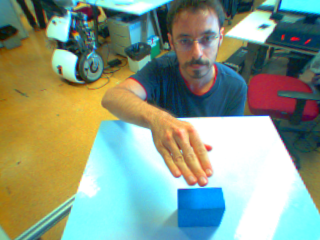
\includegraphics[width=\myWidth\linewidth]{touch-00000202}
    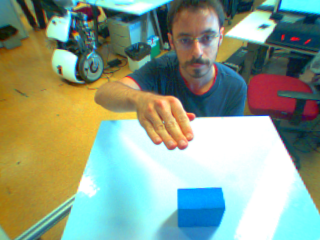
\includegraphics[width=\myWidth\linewidth]{touch-00000203}
    \label{fig:action_examples:touch}
  } % end subfloat
  \caption{Examples of human actions from the point of view of the robot}
  \label{fig:action_examples}
\end{figure*}

\section{Proposed Approach}

\begin{figure}
  \tikzstyle{affnode} = [ellipse, draw, thick]%fill=gray!20, thick]%node distance=1cm, text width=6em, text centered, minimum height=4em, thick]
  \tikzstyle{wordnode} = [ellipse, draw, thick]
  \tikzstyle{group} = [rectangle, draw, black, thick]%, inner sep=0.5cm
  \tikzstyle{dashedgroup} = [rectangle, draw, inner sep=0.6cm, dashed, rounded corners, black]
  \tikzstyle{dottedgrouptrapezium} = [trapezium, draw, dotted, rounded corners, black]
  \tikzstyle{affarrow} = [->, thick, >=stealth']%, shorten >=2pt]%, shorten >=2pt]
    \centering
    \begin{tikzpicture}
      % single nodes
      \node[affnode] (g1) {$g_1$};
      \node[affnode, right of=g1] (g2) {$g_2$};
      \node[right of=g2] (gdots) {$\dots$};
      \node[group, fit=(g1) (g2) (gdots),label=above:Gesture Features] (gestures) {};
      \node[affnode, below of=gestures] (actions) [below=1cm] {Actions};
      \node[affnode, right of=actions] (f1) [right=1.6cm] {$f_1$};
      \node[affnode, right of=f1] (f2) {$f_2$};
      \node[right of=f2] (fdots) {$\dots$};
      \node[affnode, below of=f1] (e2) [below=0.7cm] {$e_2$};
      \node[affnode, left of=e2] (e1) {$e_1$};
      \node[right of=e2] (edots) {$\dots$};
      \node[wordnode, below of=e1] (w1)  [below=0.7cm] {$w_1$};
      \node[wordnode, right of=w1] (w2) {$w_2$};
      \node[right of=w2] (wdots) {$\dots$};
      % groups
      \node[group, fit=(f1) (f2) (fdots),label=above:Object Features] (features) {};
      \node[group, fit=(e1) (e2) (edots),label=above:Effects] (effects) {};
      \node[group, fit=(w1) (w2) (wdots),label=above:Words] (words) {};
      \node[dashedgroup, fit=(actions) (features) (effects) (words),label={[shift={(0:2.2)}]above:\AffWords{} model}]{};
      % arrows
      \draw[affarrow] (actions) -- ([xshift=-30pt]effects.north);
      \draw[affarrow] (actions) to [out=260,in=150] (words.west);
      \draw[affarrow] (features) -- ([xshift=20pt]effects.north);
      \draw[affarrow] ([xshift=20pt]features.south) to [out=280,in=30] (words.east);
      \draw[affarrow] ([xshift=30pt]effects.south) -- ([xshift=30pt]words.north);
      % extra
      %\node[affnode, above of=actions] (gestures) [above=1cm] {Gesture Features};
      \draw[affarrow] (actions) -- (gestures);
      \node[dashedgroup, fit=(actions) (gestures),label=above:Gesture/Action recognition]{};
    \end{tikzpicture}
  \caption{Abstract representation of the probabilistic dependencies in the model.}
    \label{fig:model}
\end{figure}
The purpose of
%the proposed approach
our work
is to model the development of language learning from a first, self-centered, individualistic phase to a second, socially aware phase.
In the first phase the system learns by manipulating objects in its environment in a similar way as in~\cite{salvi:2012:smcb}.
In this phase, it learns to associate spoken descriptions to the combination of its actions, object properties and effects, thus grounding the meaning of words in what we call affordances.
In the second phase, the system turns to observing human actions of a similar nature as the ones explored in the first phase. Some examples are shown in Fig.~\ref{fig:action_examples}.
The robot reuses the experience acquired in the first phase to interpret the new observations and to address the correspondence problem between its own actions and the actions performed by the human.
In this phase human movements are interpreted and classified with similar methods as in~\cite{saponaro:2013:crhri}.

Our assumptions are the following:
we assume that the robot possesses visual segmentation and geometric reasoning capabilities, meaning that it is able to segment the~(potentially multiple) regions of interest corresponding to the physical objects of the world from the background~(e.g., a planar surface such as a table) and to determine their positions.
In addition, we assume that a depth sensor is available and positioned near the robot, in order to estimate the~3D coordinates of the limbs of the human, used to infer the action.

Fig.~\ref{fig:model} illustrates the probabilistic dependencies in the complete model and will be detailed in the following subsections.
The key to our approach is the existence of the discrete variable Action, the value of which is known to the robot in the ego-centric phase of learning, but must be inferred from observation in the social phase.
In the social phase, this variable links all the other observable variables, that is, human gesture features, object properties, effect variables and words.
This allows the robot to:
\begin{itemize}
\item use language in order to determine the mapping between human and own gestures/actions, and learn the corresponding perceptual models;
\item in many cases, use the affordance variables to infer the above mapping even in the absence of verbal descriptions;
\item once the perceptual models for human gesture/actions are acquired, use the complete model to do inference on any variable given some evidence.
\end{itemize}
In the following sections, first we give details on the probabilistic models enclosed in the \AffWords{} model box in Fig.~\ref{fig:model}.
Then, we describe the Gesture/Action recognition method.
Finally, we describe the way in which we combine evidence from the two models.
%We consider three \emph{manipulative gestures} corresponding to physical actions performed by agent(s) onto objects on a table~(see Fig.~\ref{fig:experimental_setup}): grasp, tap, and touch.
%Our proposed model performs probabilistic reasoning on the effects of these actions onto the objects of the world, and on the co-occurring verbal description of the experiments.

%A possible representation of the probabilistic dependencies that the robot needs to acquire in order to associate other people's actions to verbal descriptions is depicted in Fig.~\ref{fig:model:ideal}.
%The intended actions result in movements of the body that can be measured in terms of \emph{gesture features}.
%These movements, in turn, may determine some \emph{effects} on the surroundings, expressed by a number of relevant measurable variables.
%Those effects are also determined by the particular \emph{object features} associated with the objects that are involved in the action and that are also observable.
%Finally, an observer composes a verbal description of the situation based on all the observable variables.
%
%By combining the affordance model in \cite{salvi:2012:smcb} and the gesture recognition system in \cite{saponaro:2013:crhri}, however, we need to do some simplifying assumptions, that are depicted in Fig.~\ref{fig:model:our}.
%The main difference is that, in the learning phase in \cite{salvi:2012:smcb}, the intended action was known to the robot.
%The robot could, therefore, learn direct dependencies between the actions and the other variables in the \affwords{} model depicted in the corresponding dashed box in Fig.~\ref{fig:model:our}.
%Although some of the effect variables refer to the robot's arm movements, this information was not rich enough to recognize each particular gesture and could therefore not be used directly to interpret other people's behavior.
%
%This limitation can be partly overcome by the gesture/action recognition model of~\cite{saponaro:2013:crhri}, which can recover the particular intended action from the gesture features.
%Consequently, the relationship between Gesture Features, Object Features, Effects and Words, that we described earlier, is mediated by the Actions variable in our model.
%The combination of the two models is our main contribution, and allows us to relax the assumption made in \cite{salvi:2012:smcb} that the action is known during the learning phase.
%
%In the remainder of this section, we give details about the \affwords{} model, about the gesture/action recognition model employed in the study, and about the method that we employ to perform probabilistic inference by merging the information provided by those two models.

%BELOW IS THE GLU TEXT

%In this paper, we combine (1)~the robot affordance model of~\cite{salvi:2012:smcb}, which associates verbal descriptions to the physical interactions of an agent with the environment, with (2)~the gesture recognition system of~\cite{saponaro:2013:crhri}, which infers the type of action from human user movements.
%We consider three \emph{manipulative gestures} corresponding to physical actions performed by agent(s) onto objects on a table~(see Fig.~\ref{fig:experimental_setup}): grasp, tap, and touch.
%We reason on the effects of these actions onto the objects of the world, and on the co-occurring verbal description of the experiments. In the complete framework, we will use \acfp{BN}, which are a probabilistic model that represents random variables and conditional dependencies on a graph, such as in Fig.~\ref{fig:model}. One of the advantages of using \acp{BN} is that their expressive power allows the marginalization over any set of variables given any other set of variables.

%Our main contribution is that of extending~\cite{salvi:2012:smcb} by relaxing the assumption that the action is known during the learning phase.
%This assumption is acceptable when the robot learns through self-exploration and interaction with the environment, but must be relaxed if the robot needs to generalize the acquired knowledge through the observation of another~(human) agent.
%We estimate the action performed by a human user during a \hr{} collaborative task, by employing statistical inference methods and \acp{HMM}. This provides two advantages. First, we can infer the executed action during training. Secondly, at testing time we can merge the action information obtained from gesture recognition with the information about affordances.

\subsection{\AffWords{} Modeling}
\label{sec:bn}
Following the method adopted in~\cite{salvi:2012:smcb}, we use a Bayesian probabilistic framework to allow a robot to ground the basic world behavior and verbal descriptions associated to it.
All variables in the model are discrete or are discretized from continuous sensory variables through clustering in a preliminary learning phase.
Details on the variable definition and possible values are given in Table~\ref{tab:bnsymb}.
Note that the name of the values have been assigned by us arbitrarily to the clusters, for the sake of making the results more human-interpretable.
However, the robot has no prior knowledge about the meaning of these clusters.

\begin{table}
    \centering
    \caption{The symbolic variables of the \acl{BN} (from~\cite{salvi:2012:smcb}), with the corresponding discrete values obtained from clustering during robot exploration of the environment.}
    \label{tab:bnsymb}
    \begin{tabular}{cp{3.3cm}l}
    \toprule
    symbol & name: description     & values \\
    \midrule
    $a$ & Action: motor action          & grasp, tap, touch \\
    \midrule
    $f_1$ & Color: object color   & blue, yellow, green1, green2 \\
    $f_2$ & Size: object size     & small, medium, big \\
    $f_3$ & Shape: object shape    & sphere, box \\
    \midrule
    $e_1$ & ObjVel: object velocity & slow, medium, fast \\
    $e_2$ & HandVel: robot hand velocity & slow, fast \\
    $e_3$ & ObjHandVel: relative \objecthand{} velocity & slow, medium, fast \\
    $e_4$ & Contact: object hand contact & short, long \\
    \midrule
    $w_1$--$w_{49}$ & presence of each word in the verbal description & true, false \\
    \bottomrule
    \end{tabular}
\end{table}

To simplify the notation, we can group the affordance and word variables according to their use for the following descriptions: action variable~$A = \{a\}$, object feature variables~$F=\{f_1, f_2, \dots\}$, effect variables~$E=\{e_1, e_2, \dots\}$ and word variables~$W = \{w_1, w_2, \dots\}$.
The \ac{BN} model relates all these variables by means of the joint probability distribution~$\pbn(A, F, E, W)$, sketched by the \AffWords{} model box in Fig.~\ref{fig:model}.
The dependency structure and the model parameters are estimated by the robot in an ego-centric way through interaction with the environment, as in~\cite{salvi:2012:smcb}.
As a consequence, during learning, the robot knows what action it is performing with certainty, and the variable~$A$ assumes a deterministic value.
During inference, the probability distribution on the variable~$A$ can be inferred from evidence on the other nodes.
For example, if the robot is asked to make a spherical object roll, it will be able to select the action tap as most likely to obtain the desired effect, based on previous experience.

\newcommand{\myscalefactor}{0.8}

\newcommand{\shapeOfHmmState}{circle} % CR-HRI style
%\newcommand{\shapeOfHmmState}{rectangle} % Bishop style?

\newcommand{\standardhmm}[1]{
    \node[draw,\shapeOfHmmState] (hmm#1s1) {$s_1$};
    \node[draw,\shapeOfHmmState, right of=hmm#1s1] (hmm#1s2) {$s_2$};
    \node[\shapeOfHmmState, right of=hmm#1s2] (hmm#1s3) {\dots};
    \node[draw,\shapeOfHmmState, right of=hmm#1s3] (hmm#1s4) {$s_Q$};
    \node[left of=hmm#1s1]  (invisible1) {};
    \node[right of=hmm#1s4] (invisible2) {};
    \path[->] (hmm#1s1) edge (hmm#1s2);
    \path[loop above] (hmm#1s1) edge (hmm#1s1);
    \path[->] (hmm#1s2) edge (hmm#1s3);
    \path[loop above] (hmm#1s2) edge (hmm#1s2);
    \path[dashed] (hmm#1s2) -- (hmm#1s3);
    \path[->] (hmm#1s3) edge (hmm#1s4);
    \path[loop above] (hmm#1s4) edge (hmm#1s4);
    %\path[->] (hmm#1s4) edge[bend left] (hmm#1s1);
    \path[->] (invisible1) edge (hmm#1s1);
    \path[->] (hmm#1s4) edge (invisible2);
}

\newcommand{\modeltwo}{
  \begin{tikzpicture}[scale=\myscalefactor, every node/.style={scale=\myscalefactor}]
  \matrix (M) [matrix of nodes, ampersand replacement=\&] {%
    grasp gesture HMM \& \standardhmm{1} \\
    tap gesture HMM \& \standardhmm{2} \\
    touch gesture HMM \& \standardhmm{3} \\
    %garbage \& \standardhmm{4} \\
  };
  \end{tikzpicture}
}

\begin{figure}
  \centering
  \modeltwo
  \caption{Structure of the \acp{HMM} used for human gesture recognition, adapted from~\cite{saponaro:2013:crhri}. In this work, we consider three independent, multiple-state \acp{HMM}, each of them trained to recognize one of the considered manipulation gestures of Figs.~\ref{fig:action_examples:grasp}, \ref{fig:action_examples:tap}, \ref{fig:action_examples:touch} respectively.}
  \label{fig:hmms}
\end{figure}

\subsection{Gesture/Action Recognition}
When observing a human performing actions, the value of the action variable~$A$ is not known to the robot neither during learning nor during inference.
During learning, we assume that the robot has not yet acquired a perceptual model of the gestures associated to the human actions.
The value of~$A$ can, however, be inferred either from a verbal description of the scene or from the other affordance nodes through the \AffWords{} model described earlier.

For example, similarly to Sec.~\ref{sec:bn}, the \AffWords{} model predicts that performing a tap action on a spherical object will result in high velocity of the object.
If the human performs an unknown action on a spherical object and obtains a high velocity, the robot will be able to infer that the action is most probably a tap, although it was not able to recognize the gesture associated with this action.

This information can be used to train a gesture/action recognition system similar to the one in~\cite{saponaro:2013:crhri}.
The system, depicted in Fig.~\ref{fig:hmms} and corresponding to the Gesture/Action recognition block in Fig.~\ref{fig:model}, is based on \acp{HMM} with Gaussian mixture models as emitting probability distributions.
%The gesture recognition models are represented in Fig.~\ref{fig:hmms}, and correspond to the Gesture/Action recognition block in Fig.~\ref{fig:model}.
%As for the gesture recognition \acsp{HMM}, we use the models that we previously trained in~\cite{saponaro:2013:crhri} for spotting the manipulation-related gestures under consideration.
Our input features are the~3D coordinates of the tracked human hand indicated by the~$g_i$ variables in Fig.~\ref{fig:model}.
The coordinates are obtained with a commodity depth sensor, then transformed to be centered on the person torso~(to be invariant to the distance between the user and the sensor) and normalized to account for variability in amplitude~(to be invariant to wide/emphatic vs narrow/subtle executions of the same action).

The model for each gesture/action is a
%so-called
left-to-right \ac{HMM}, where the transition model between the discrete states~$\mathcal{S} = \{s_1, \dots, s_Q\}$ is structured so that states with lower index represent events that occur earlier in time.
%set of (hidden) discrete states~$\mathcal{S} = \{s_1, \dots, s_Q\}$ which model the temporal phases comprising the dynamic execution of the gesture, and by a set of parameters~$\lambda = \{ A, B, \Pi \}$, where~$A = \{ a_{ij} \}$ is the transition probability matrix, $a_{ij}$ is the transition probability from state~$s_i$ at time~$t$ to state~$s_j$ at time~$t+1$, $B = \{ f_i \}$ is the set of $Q$~observation probability functions~(one per state~$i$) with continuous mixtures of Gaussian values, and~$\Pi$ is the initial probability distribution for the states.

Although not expressed so far in the notation, the continuous variables~$g_i$ are measured at regular time intervals.
At a certain time step~$n$, the feature vector can be expressed as~$\bm{g}[n] = \{g_1[n], \dots, g_D[n]\}$.
The input to the model is a sequence of~$N$ such feature vectors~$\bm{g}[1], \dots, \bm{g}[N]$ that we call for simplicity~$G_1^N$, where~$N$ can vary for every recording.

At recognition~(testing) time, we can use the models to estimate the likelihood of a new sequence of observations~$G_1^N$, given each possible gesture/action by means of the \FB{} inference algorithm.
%We can express this likelihood as $\mathcal{L}_\text{HMM}(G_1^N \given A)$, where $a$ is one of the possible actions.
We can express this likelihood as $\mathcal{L}_\text{HMM}(G_1^N \given A=a_k)$, where $a_k$ is one of the possible actions.
By normalizing the likelihoods, assuming that the gestures are equally likely \emph{a priori}, we can obtain the posterior probability of the action given the sequence of observations as
\begin{equation} \label{eq:phmm_action}
  \phmm(A=a_k \given G_1^N) = \frac{\mathcal{L}_\text{HMM}(G_1^N \given A=a_k)}{\sum_h \mathcal{L}_\text{HMM}(G_1^N \given A=a_h)}.
\end{equation}

\subsection{Combining the \acs{BN} with Gesture \acsp{HMM}}
\label{sec:combination}
Once learned, the two models described above define two probability distributions over the relevant variables for the problem:
$\pbn(A, F, E, W)$ and~$\phmm(A \given G_1^N)$.
The goal during inference is to merge the information provided by both models and estimate~$\pcomb(A, F, E, W \given G_1^N)$, that is, the joint probability of all the affordance and word variables, given that we observe a certain gesture/action performed by the human.

To simplify the notation, we call $X = \{A, F, E, W\}$ the set of affordance and word variables~$\{a, f_1, f_2, \dots, e_1, e_2, \dots, w_1, w_2, \dots\}$.
During inference, we have a (possibly empty) set of observed variables~$\xobs \subseteq X$, and a set of variables $\xinf \subseteq X$ on which we wish to perform the inference.
In order for the inference to be non-trivial, it must be~$\xobs \cap \xinf = \varnothing$, that is, we should not observe any inference variable.
According to the \ac{BN} alone, the inference will compute the probability distribution of the inference variables~$\xinf$ given the observed variables~$\xobs$ by marginalizing over all the other (latent) variables $\xlat = X \setminus (\xobs \cup \xinf)$, where~$\setminus$~is the set difference operation:
\begin{equation*}
 \pbn(\xinf \given \xobs) = \sum_{\xlat} \pbn(\xinf, \xlat \given \xobs).
\end{equation*}

If we want to combine the evidence brought by the \ac{BN} with the evidence brought by the \ac{HMM}, there are two cases that can occur:
\begin{enumerate}
\item the variable action is included among the inference variables: $A \in \xinf$, or

\item the variable action is not included among the inference variables: $A \in \xlat$.
\end{enumerate}

Here, we are excluding the case where we observe the action directly~($A\in \xobs$) for two reasons: firstly, this would correspond to the robot performing the action itself, whereas we are interested in interpreting other people's actions;
secondly, this would make the evidence on the gesture features~$G_1^N$ irrelevant, because in the model in Fig.~\ref{fig:model}, there is a tail-to-tail connection from~$G_1^N$ to the rest of the variables through the action variable, which means that, given the action, all dependencies to the gesture features are dropped.

The two cases enumerated above can be addressed separately when we do inference.
In the first case, we call~$\xinf^\prime$ the set of inference variables excluding the action~$A$, that is, $\xinf = \{\xinf^\prime, A\}$.
We can write:
\begin{align} \label{eq:fusion_excluding_action}
  & \pcomb(\xinf \given  \xobs, G_1^N) = \pcomb(A, \xinf^\prime \given  \xobs, G_1^N)= \nonumber \\
  &= \sum_{\xlat} \pcomb(A, \xinf^\prime, \xlat \given \xobs, G_1^N)= \nonumber\\
  &= \sum_{\xlat} \left[\pbn(A, \xinf^\prime, \xlat \given \xobs, G_1^N)\right. \nonumber \\[-4mm]
    & \mspace{80mu} \left.\phmm(A, \xinf^\prime, \xlat \given \xobs, G_1^N)\right]= \nonumber \\
  &= \left[\sum_{\xlat} \pbn(A, \xinf^\prime, \xlat \given \xobs)\right] \phmm(A \given G_1^N) \nonumber \\
  &= \pbn(\xinf \given \xobs) \phmm(A \given G_1^N).
\end{align}
This means that we can evaluate the two models independently, then multiply the distribution that we obtain from the \ac{BN}~(over all the possible value of the inference variables) by the \ac{HMM} posterior for the corresponding value of the action.

In the second case, where the action is among the latent variables, we define, similarly, $\xlat = \{A, \xlat^\prime\}$, and we have:
\begin{align} \label{eq:fusion_including_action}
  & \pcomb(\xinf \given \xobs, G_1^N) = \nonumber \\
  &= \sum_{\{A,\xlat^\prime\}} \pcomb(\xinf, A, \xlat^\prime \given \xobs, G_1^N)= \nonumber \\
  &= \sum_{\{A,\xlat^\prime\}} \left[\pbn(\xinf, A, \xlat^\prime \given \xobs, G_1^N)\right. \nonumber \\[-4mm]
    & \mspace{100mu} \left.\phmm(\xinf, A, \xlat^\prime \given \xobs, G_1^N)\right]= \nonumber \\[2mm]
  &= \sum_{\{A,\xlat^\prime\}} \left[\pbn(\xinf, A, \xlat^\prime \given \xobs) \phmm(A \given G_1^N)\right] \nonumber \\
  &= \sum_{A}\left[\phmm(A \given G_1^N)\sum_{\xlat^\prime} \pbn(\xinf, A, \xlat^\prime \given \xobs)\right] \nonumber \\
  &= \sum_{A}\left[\phmm(A \given G_1^N) \pbn(\xinf, A \given \xobs)\right].
\end{align}
This time, we first need to use the \ac{BN} to do inference on the variables~$\xinf$ and~$A$, and then we marginalize out the action variable~$A$ after having multiplied the probabilities by the \ac{HMM} posterior.

\subsection{Generation and Scoring of Verbal Descriptions}
\label{sec:approach:verbal}

In order to illustrate the language capabilities of the model, we use the \ac{CFG} described in Appendix~\ref{appendix:grammar} to generate written descriptions of the robot observations on the basis of the probability distributions of the words inferred by the model.
Note that this grammar is defined here with the only purpose to interpret the probability distributions over the words.
The grammar was neither used in the speech recognition system, nor in learning the associations of the spoken utterances to the affordance variables.
In the model described in~\cite{salvi:2012:smcb}, the speech recognizer used a free loop of words with uniform prior distribution over the words, and the Bayesian model used a bag-of-words assumption, thus disregarding any syntactic information about the spoken descriptions.

In the current study, by merging the \AffWords{} model and the gesture/action recognition model, we allow the robot to \emph{reinterpret} the concepts it has learned in the self-centered phase, but we do not add any new words to the model.
Consequently, the descriptions that the model generates when observing humans use the same words to describe the agent.

The textual descriptions are generated as follows: given some evidence~$\xobs$ that we provide to the model and some human observation features~$G_1^n$ extracted from frames~$1$ to~$n$, we extract the generated word probabilities
$P(w_i \given \xobs, G_1^n)$.
We generate~$N$ sentences randomly from the \ac{CFG} using the \texttt{HSGen} tool from HTK~\cite{young:htkbook}.
Then, the sentences are re-scored according to the log-likelihood of each word in the sentence, normalized by the length of the sentence:
\begin{equation} \label{eq:sentence_score}
  \text{score}(s_j \given \xobs, G_1^n) = \frac{1}{L_j} \sum_{k=1}^{L_j} \log P(w_{jk} \given \xobs, G_1^n),
\end{equation}
where~$s_j$ is the~$j$th sentence,~$L_j$ is the number of words in the sentence~$s_j$, and~$w_{jk}$ is the~$k$th word in the sentence~$s_j$.
Finally, an $N$-best list of possible descriptions is produced by sorting the scores.

%GLU TEXT
%
%In this study we wish to generalize the model of~\cite{salvi:2012:smcb} by observing external~(human) agents, as shown in Fig.~\ref{fig:experimental_setup}. For this reason, the full model is now extended with a perception module capable of inferring the action of the agent from visual inputs. This corresponds to the Gesture \acp{HMM} block in Fig.~\ref{fig:model}. The \AffWords{} \acf{BN} model and the Gestures \acp{HMM} may be combined in different ways~\cite{pan:2006:ictai}:
%\begin{enumerate}
%\item the Gesture \acp{HMM} may provide a hard decision on the action performed by the human~(i.e., considering only the top result) to the \ac{BN},
%
%\item the Gesture \acp{HMM} may provide a posterior distribution~(i.e., soft decision) to the \ac{BN},
%
%\item if the task is to infer the action, the posterior from the Gesture \acp{HMM} and the one from the \ac{BN} may be combined as follows, assuming that they provide independent information:
%\begin{equation*}
%p(A) = \phmm(A) \, \pbn(A).
%\end{equation*}
%\end{enumerate}
%

\bigskip

In the experimental section, we will show that what the robot has learned subjectively or alone~(by self-exploration, knowing the action identity as a prior~\cite{salvi:2012:smcb}), can subsequently be used when observing a new agent~(human), provided that the actions can be estimated with Gesture \acp{HMM} as in~\cite{saponaro:2013:crhri}.
In addition, we will show the emergence of language phenomena within the generated verbal descriptions.
